\section{Lineare Zeitinvariante Systeme (LZI)}

Für \textbf{lineare, zeitinvariante Systeme} gibt es viele Analyse- und Synthesemethoden für Regler \\
\textrightarrow\ Für \textbf{Entwurf} von Reglern gewünscht

\vspace{0.2cm}

Reale Systeme sind hingegen \textbf{nichtlinear und zeitvariant} \\
\textrightarrow\ Für \textbf{Simulation / Validierung} von Reglern gewünscht 


\subsection{Linearität (Definition)}{77}

Gegeben sei ein System 
$$ \Phi: u(t) \rightarrow y(t) \qquad y(t) = \Phi(u(t))$$
Wenn das System das \textbf{Superpositionsprinzip erfüllt}, so ist das System \textbf{linear} \\
\textrightarrow\ 'Es kommt nich auf die Reihenfolge der Operationen an'

$$ \boxed{ \cgn{ \Phi( \alpha_A \cdot u_A(t) + \alpha_B \cdot u_B(t)) } = \cbl{ \alpha_A \cdot \Phi(u_A(t)) + \alpha_B \cdot \Phi(u_B(t)) } } $$

\begin{center}
	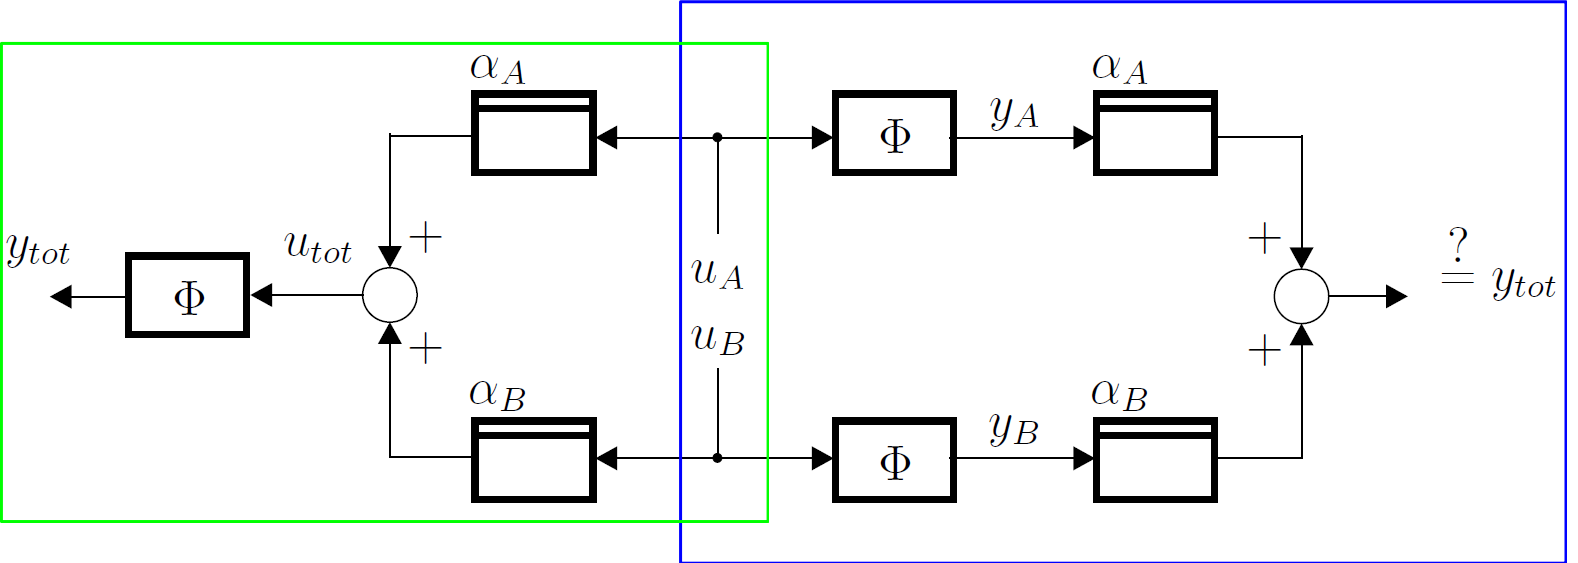
\includegraphics[width=0.9\columnwidth]{images/pruefung_linearitaet.png} 
\end{center}

Ein guter Test ist, ein \textbf{'Gegenbeweis'} mit der Bedingung $u(t) = 0$ 
$$ \Phi(0 \cdot u(t)) = 0 \cdot \Phi(u(t)) = 0 $$
\textrightarrow\ Wenn dieser Test \textbf{fehlschlägt} ist das System \textbf{nichtlinear}!


\subsection{Lineare Systeme}

Alle Systeme, die mit \textbf{Differentialgleichungen mit konstanten Koeffizienten} beschrieben werden, sind linear 
$$ \boxed{ a_n y(t)^{(n)} + ... + a_1 \dot{y}(t) + a_0 y(t) = b_m u(t)^{(m)} + ... + b_1 \dot{u}(t) + b_0 u(t) } $$
\textrightarrow\ Zeitverschiebung ändert nichts an der Linearität des Systems!


\subsubsection{Beispiele linearer Systeme}

\begin{minipage}[t]{0.4\columnwidth}
	\begin{tabular}{lll}
		\tabitem Verstärkung 			& $y(t) = K \cdot u(t)$ 					\\
		\tabitem Integrator 			& $\dot{y}(t) = u(t)$ 						
	\end{tabular}
\end{minipage}
\hfill
\begin{minipage}[t]{0.58\columnwidth}
	\begin{tabular}{lll}
		\tabitem Differenzierer 		& $y(t) = \dot{u}(t)$ 						\\
		\tabitem $\text{PT}_1$-Glied 	& $T \, \dot{y}(t) + y(t) = K \cdot u(t)$ 
	\end{tabular}
\end{minipage}


\subsection{Zeitinvarianz (Defintion)}{79}

Gegeben sei ein System 
$$\Phi: u(t) \rightarrow y(t) \qquad y(t) = \Phi(u(t))$$

Ist das System zeitinvariant, so gilt
$$ \boxed{ \Phi(u(t-T_t)) = y(t - T_t) \quad \forall \; T_t } $$
\textrightarrow\ Die Antwort des Systems ist unabhängig davon, zu welchem Zeitpunkt der Eingang anliegt


\subsubsection{Eigenschaften zeitvarianter Systeme}

\begin{itemize}
	\setlength\itemsep{5pt}

	\item Sie \textbf{können} linear sein, weil Superpositionsprinzip möglich \\
		$\Phi( \alpha_A \cdot u_A(t) + \alpha_B \cdot u_B(t), \, t)  \, = \, \alpha_A \cdot \Phi(u_A(t), \, t) + \alpha_B \cdot \Phi(u_B(t), \, t)$ \\
		$\Phi( \alpha_A \cdot u_A(t) + \alpha_B \cdot u_B(t), \, t - T_t)  \, = \, \alpha_A \cdot \Phi(u_A(t), \, t - T_t) + \alpha_B \cdot \Phi(u_B(t), \, t - T_t)$ 

	\item Oft ist nicht klar, ob ein Effekt zeitvariant oder nichtlinear ist
	\begin{itemize}
		\item Verschleiss in Abängigkeit der Beanspruchung \textrightarrow\ nichtlinear
		\item Verschleiss in Abängigkeit der Zeit (Alterung) \textrightarrow\ zeitvariant
	\end{itemize}
		

	\item Die Behandlung zeitvarianter Systeme ist manchmal einfacher als nichtlineare Systeme 
\end{itemize}


\subsection{Umgang mit LZI-Systemen}

Wir beschäftigen uns mit LZI-Systemen, weil... 

\vspace{0.1cm}
\begin{itemize}
	\item Setzt man Systeme aus LZI Systemen zusammen, so entsteht wieder ein LZI-System 
	\item Bei seriegeschalteten LZI-Systemen kann die Reihenfolge getauscht werden
	\item Für LZI-Systeme ist ein Frequenzbereich definiert \\
 		\textrightarrow\ Sinusförmige Signale ändern Amplitude und Phase, allerdings nicht die Frequenz! \\
		\textrightarrow\ Beschreibung des LZI-Systems mittels Frequenzgang $G(\jimg \omega)$, welcher Reaktion des Systems auf eine bestimmte Frequenz beschreibt \\
\end{itemize}

Amplitudenänderung $| G(\jimg \omega) |$ ; Phasenänderung $\arg( G(\jimg \omega ))$ 


\subsection{Serieschaltung von LZI-Systemen}{82}
\label{Serieschaltung von LZI-Systemen}

\textbf{Die Reihenfolge der Blöcke darf getauscht werden}
 
\begin{center}
	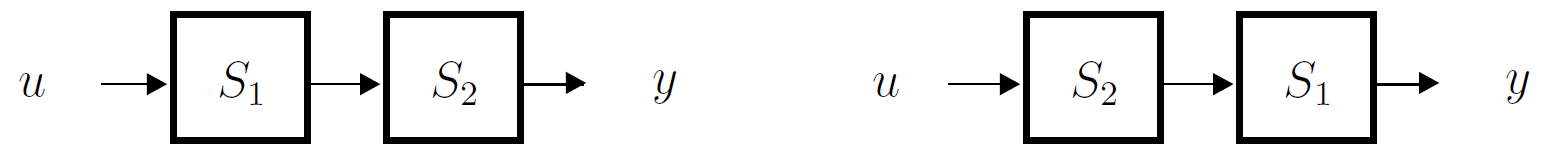
\includegraphics[width=0.85\columnwidth]{images/bloecke_tauschen.png}
\end{center}

Blöcke dürfen \textbf{verschoben werden}, müssen allerdings mit ihrer \textbf{Umkehrfunktion kompensiert werden}, um das Gesamtsystem nicht zu verändern

\begin{center}
	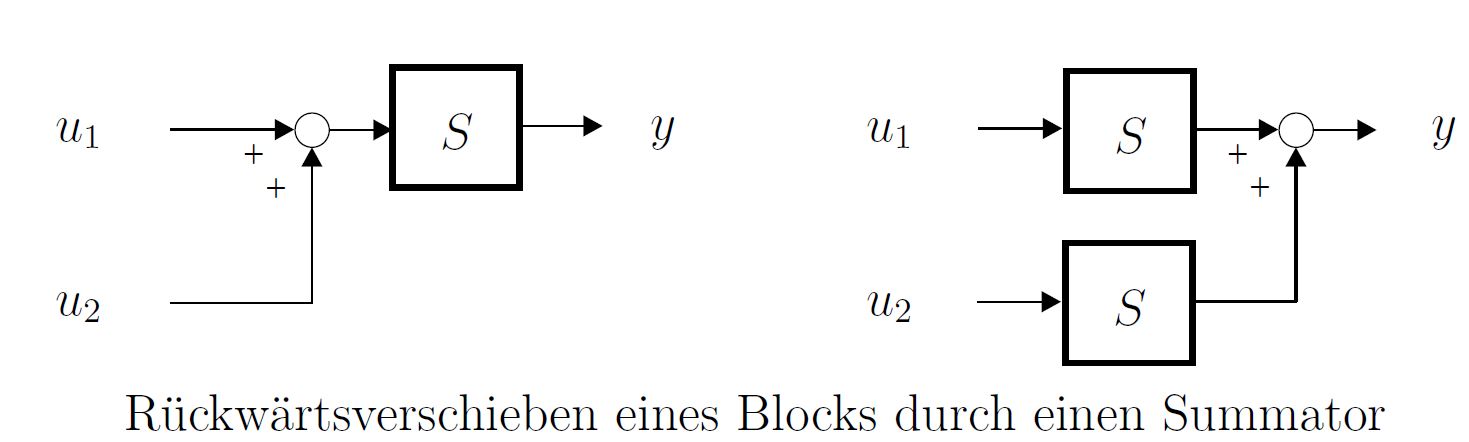
\includegraphics[width=0.73\columnwidth]{images/bloecke_schieben_1.png}
	\vspace{0.2cm}

	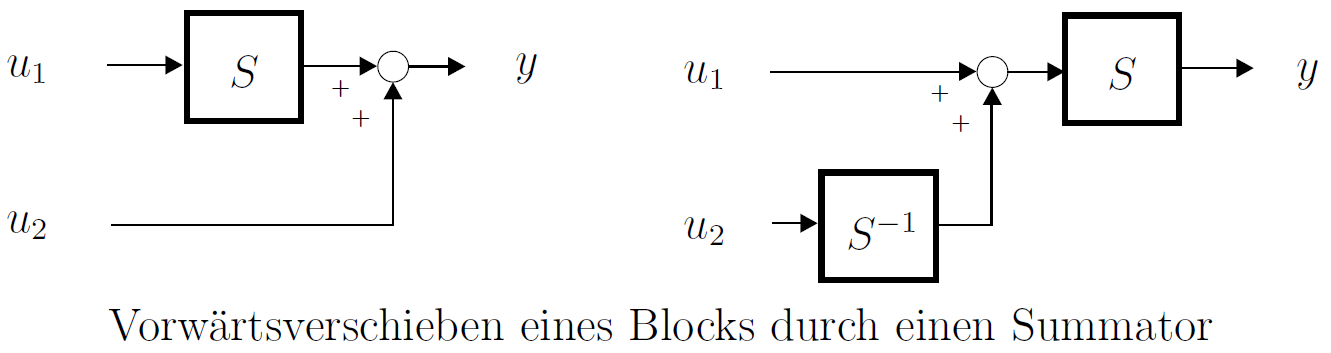
\includegraphics[width=0.73\columnwidth]{images/bloecke_schieben_2.png}
	\vspace{0.2cm}

	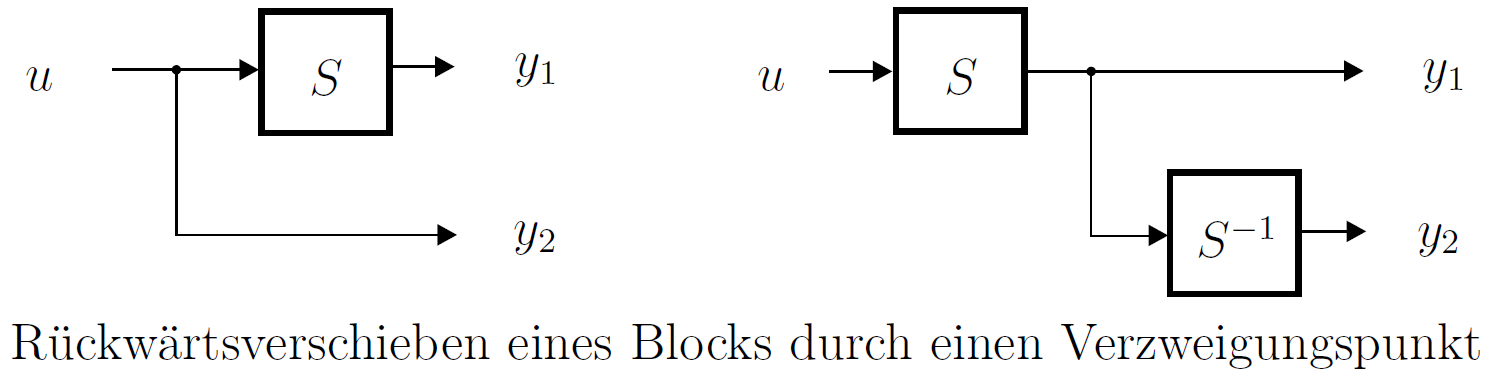
\includegraphics[width=0.73\columnwidth]{images/bloecke_schieben_3.png} 
\end{center}

